\chapter[Revisão Bibliográfica]{Revisão Bibliográfica}
\label{chap:revisao_bibliografica}
\thispagestyle{empty}

Este capitulo é divido em duas seções que visam apresentar os conceitos necessários para a compreensão deste PFC.
Na primeira seção são aprensados conceitos para uma modelagem matemática da dinâmica de um veiculo em baixas velocidades.
São apresentado na segunda seção uma introdução à teoria de controle ótimo e a utilização de programação não linear na solução
de problemas de controle ótimo.

\section{Modelo do veículo}
\label{sec:modelo}

Um modelo matemático, ou apenas modelo, é um conjunto de equações que descreve de forma adequada o comportamento de um sistema que deseja-se estudar.
Uma forma usual de classificação dos métodos de modelagem é separa-los nas categorias: modelagem caixa branca, modelagem caixa preta e modelagem
caixa cinza.
A modelagem caixa branca, também conhecida como modelagem conceitual, consiste na aplicação princípios fundamentais e por isso exige um conhecimento
da natureza do sistema.
A modelagem caixa preta, ou modelagem empírica, é baseada na aplicação de técnicas de identificação de sistemas que exigem pouco ou
nenhum conhecimento do sistema.
Já na modelagem caixa cinza sáo utilizadas técnicas que estão entre a modelagem caixa branca e a modelagem caixa preta\cite{book:Aguirre}.

Nessa seção o método de modelagem aplicado é de modelagem caixa branca. A partir da aplicação da segunda lei de Newton no
veiculo representado no diagrama da Figura \ref{fig:diag_forcas_veiculo}, obtém-se a equação que descreve a dinâmica longitudinal do mesmo

\begin{equation}
	\label{eq:SomaForcas}
	m \cdot \dot v	= F_t - (F_a +	F_g + F_p)
	\enspace,
\end{equation}

em que $m$ é a massa total, $v$ é a velocidade, $F_{t}$ é a propulsão feita pelo motor subtraída as perdas do sistema de transmissão, $F_{a}$ é o
arrasto aerodinâmico, $F_g$ é a componente do peso que esta direção da velocidade e $F_{p}$ é a resistência ao rolamentos dos pneus no pista.
Os modelos que descrevem a forças $F_{a}$, $F_g$, $F_{p}$ e $F_{t}$ estão apresentados nas subseções a seguir.

\begin{figure}[H]
	\centering
	\caption{Diagrama de forças de um veículo em movimento}
	\label{fig:diag_forcas_veiculo}
	\begin{normalsize}
		\import{DescricaoProcesso/Figuras/}{diagrama_forcas_veiculo.pdf_tex}
	\end{normalsize}
	\caption*{\footnotesize Fonte: Elaborado pelo autor.}
\end{figure}

\subsection{Arrasto Aerodinâmico}
\label{subsec:arrasto_aerodinamico}

O movimento de um objeto imerso em um fluido sofre uma resistência causada por esse fluido. No
caso de veículos que se deslocando no ar, essa
resistência é chamada de arrasto aerodinâmico.
Pode-se aproximar o calculo dessa força $F_{a}$ com a equação

\begin{equation}
	\label{eq:Fa}
	F_a(v) = \frac{\rho \cdot a_f \cdot c_d \cdot v^2}{2}
	\enspace,
\end{equation}

em que $v$ é a velocidade do veiculo em relação ao vento, $\rho$ a densidade do ar, $a_{f}$ a área frontal do
veiculo e $c_{d}$ o coeficiente de arrasto aerodinâmico.
O coeficiente $c_{d}$ é um numero adimensional e depende da geometria veiculo, é determinado por meio de simulações em \textit{software} de fluido
dinâmica
computacional (CFD, do inglês \textit{computational fluid dynamics}) e/ou experimentos em túnel de vento\cite{book:guzzella2012vehicle}. Alguns
valores típicos de $C_{d}$ para diferentes tipos de
veículos são apresentados na Tabela \ref{tab:ComparacaoCD}.

\begin{table}[H]
	\centering
	\caption{Comparação do $c_{d}$ de diferentes tipos veículos}
	\rowcolors{1}{}{lightgray}
	\begin{tabular}{ll}
		\toprule
		\textbf{Veiculo} & \boldsymbol{$c_{d}$} \\
		\hline
		Carro            & 0,3 - 0,4            \\
		Ônibus           & 0,6 - 0,7            \\
		Caminhão         & 0,6 - 1,0            \\
		Moto             & 0,5 - 1,0            \\
		\bottomrule
	\end{tabular}
	\caption*{\footnotesize Fonte: Adaptado de \citeauthor{book:GroundVehicleDynamics}.}
	\label{tab:ComparacaoCD}
\end{table}

\subsection{Relevo da pista}

A componente do peso, $F_{g}$, afeta consideravelmente a dinâmica do veiculo e atua sempre que a pista não é plana. Seu modelo é a equação

\[
	F_{g}(\theta) = m \cdot g \cdot \sin(\theta)
	\enspace,
\]

que, pra pequenas inclinações, pode ser aproximado pela equação

\begin{equation}
	\label{eq:Fg}
	F_{g}(\theta) \approx  m \cdot g \cdot \theta
	\enspace,
\end{equation}

em que $m$ é a massa total do veículo, $g$ é a aceleração da gravidade e $\theta$ é a inclinação da pista expressa em
radianos\cite{book:guzzella2012vehicle}.

\subsection{Resistência ao rolamento}
\label{subsec:resistencia_rolamento}

A norma ISO 4223-1:2017 define a resistência ao rolamento de um pneu, como a energia consumida pelo pneu por unidade de distancia
percorrida. Esse consumo de energia se deve principalmente as propriedades viscoelásticas dos compostos de borracha presente no pneu.
Durante a rolagem o pneu é deformado na zona de contato entre o pneu e o pavimento, nessa zona de contato a resultante da força de reação à força
normal não
está no mesmo eixo que a força normal, Figura \ref{fig:diagramaPeneu}, de forma a gerar um força, $F_{r}$, contraria a movimentação do pneu.

\tikzset{every picture/.style={line width=0.75pt}} %set default line width to 0.75pt        
\begin{figure}[H]
    \begin{center}
        \caption{Legenda diagrama pneu}
        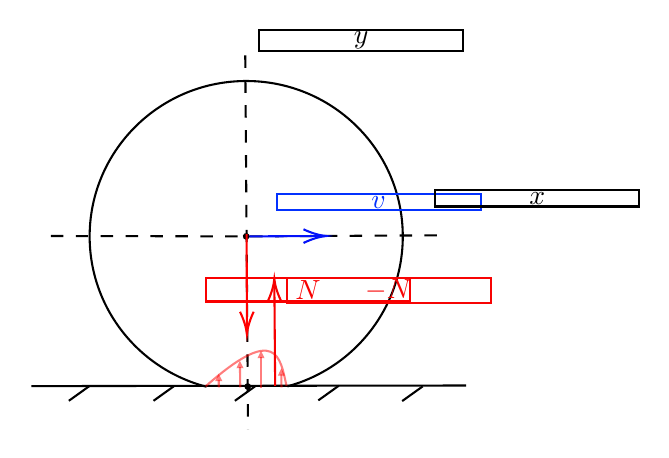
\begin{tikzpicture}[x=0.75pt,y=0.75pt,yscale=-1,xscale=1]
            %uncomment if require: \path (0,189); %set diagram left start at 0, and has height of 189

            %Straight Lines [id:da7518330174479086] 
            \draw  [dash pattern={on 4.5pt off 4.5pt}]  (6.67,90) -- (100.79,90.19) -- (193.33,89.67) ;
            %Straight Lines [id:da5592434503400421] 
            \draw	 (-2.68,162.32) -- (206.73,162.03) ;
            %Shape: Arc [id:dp1726281412706019] 
            \draw  [draw opacity=0][fill={rgb, 255:red, 8; green, 7; blue, 7 }  ,fill opacity=0 ] (81.65,162.63) .. controls (49.67,154.34) and
            (25.87,125.7) .. (25.36,91.3) .. controls (24.76,49.95) and (58.03,15.94) .. (99.69,15.33) .. controls (141.35,14.72) and (175.61,47.74) ..
            (176.22,89.08) .. controls (176.73,124) and (153.08,153.68) .. (120.62,162.44) -- (100.79,90.19) -- cycle ; \draw   (81.65,162.63) .. controls
            (49.67,154.34) and (25.87,125.7) .. (25.36,91.3) .. controls (24.76,49.95) and (58.03,15.94) .. (99.69,15.33) .. controls (141.35,14.72) and
            (175.61,47.74) .. (176.22,89.08) .. controls (176.73,124) and (153.08,153.68) .. (120.62,162.44) ;
            %Straight Lines [id:da003920177628984778] 
            \draw [color={rgb, 255:red, 4; green, 18; blue, 249 }  ,draw opacity=1 ]   (100.79,90.19) -- (137.33,90.01) ;
            \draw [shift={(139.33,90)}, rotate = 539.72] [color={rgb, 255:red, 4; green, 18; blue, 249 }  ,draw opacity=1 ][line width=0.75]
            (10.93,-3.29) .. controls (6.95,-1.4) and (3.31,-0.3) .. (0,0) .. controls (3.31,0.3) and (6.95,1.4) .. (10.93,3.29)   ;
            %Straight Lines [id:da6241641943206588] 
            \draw [color={rgb, 255:red, 0; green, 0; blue, 0 }  ,draw opacity=1 ]	(25.2,162.33) -- (15.33,169.4) ;
            %Straight Lines [id:da6421337551968986] 
            \draw [color={rgb, 255:red, 0; green, 0; blue, 0 }  ,draw opacity=1 ]	(66,162.33) -- (56.13,169.4) ;
            %Straight Lines [id:da25242184369144227] 
            \draw [color={rgb, 255:red, 0; green, 0; blue, 0 }  ,draw opacity=1 ]	(105.2,162.33) -- (95.33,169.4) ;
            %Straight Lines [id:da7965874493492349] 
            \draw [color={rgb, 255:red, 0; green, 0; blue, 0 }  ,draw opacity=1 ]	(145.4,162.13) -- (135.53,169.2) ;
            %Straight Lines [id:da2366122350933053] 
            \draw [color={rgb, 255:red, 0; green, 0; blue, 0 }  ,draw opacity=1 ]	(185.8,162.47) -- (175.93,169.53) ;
            %Straight Lines [id:da201352955590123] 
            \draw  [dash pattern={on 4.5pt off 4.5pt}]  (100.33,3) -- (101.67,183) ;
            %Straight Lines [id:da12037912623915337] 
            \draw	 (-4,15.67) ;
            %Shape: Circle [id:dp21540655765824446] 
            \draw  [color={rgb, 255:red, 0; green, 0; blue, 0 }  ,draw opacity=1 ][fill={rgb, 255:red, 0; green, 0; blue, 0 }  ,fill opacity=1 ]
            (100.45,162.53) .. controls (100.45,161.94) and (100.94,161.45) .. (101.53,161.45) .. controls (102.13,161.45) and (102.62,161.94) .. (102.62,162.53)
            .. controls (102.62,163.13) and (102.13,163.62) .. (101.53,163.62) .. controls (100.94,163.62) and (100.45,163.13) .. (100.45,162.53) -- cycle ;
            %Shape: Circle [id:dp5323977356859111] 
            \draw  [color={rgb, 255:red, 0; green, 0; blue, 0 }  ,draw opacity=1 ][fill={rgb, 255:red, 0; green, 0; blue, 0 }  ,fill opacity=1 ]
            (99.73,89.99) .. controls (99.84,89.4) and (100.4,89.01) .. (100.99,89.13) .. controls (101.58,89.24) and (101.97,89.8) .. (101.85,90.39) .. controls
            (101.74,90.98) and (101.17,91.37) .. (100.59,91.25) .. controls (100,91.14) and (99.61,90.58) .. (99.73,89.99) -- cycle ;
            %Straight Lines [id:da8962219135738276] 
            \draw [color={rgb, 255:red, 255; green, 0; blue, 0 }  ,draw opacity=1 ]   (100.99,89.13) -- (101.13,135.43) ;
            \draw [shift={(101.13,137.43)}, rotate = 269.83] [color={rgb, 255:red, 255; green, 0; blue, 0 }  ,draw opacity=1 ][line width=0.75]
            (10.93,-3.29) .. controls (6.95,-1.4) and (3.31,-0.3) .. (0,0) .. controls (3.31,0.3) and (6.95,1.4) .. (10.93,3.29)	;
            %Straight Lines [id:da7902625791767064] 
            \draw [color={rgb, 255:red, 246; green, 0; blue, 0 }  ,draw opacity=1 ][fill={rgb, 255:red, 254; green, 0; blue, 0 }  ,fill opacity=1
            ]   (114.73,162.23) -- (114.35,112.63) ;
            \draw [shift={(114.33,110.63)}, rotate = 449.56] [color={rgb, 255:red, 246; green, 0; blue, 0 }  ,draw opacity=1 ][line width=0.75]
            (10.93,-3.29) .. controls (6.95,-1.4) and (3.31,-0.3) .. (0,0) .. controls (3.31,0.3) and (6.95,1.4) .. (10.93,3.29)	;
            %Curve Lines [id:da9381909177646195] 
            \draw [color={rgb, 255:red, 255; green, 0; blue, 0 }  ,draw opacity=0.51 ]   (81.25,162.43) .. controls (115.59,132.01) and
            (117.14,148.45) .. (120.22,162.24) ;
            %Straight Lines [id:da46399317653073635] 
            \draw [color={rgb, 255:red, 255; green, 0; blue, 0 }  ,draw opacity=0.51 ]   (87.58,162.88) -- (87.55,159.32) ;
            \draw [shift={(87.53,156.32)}, rotate = 449.5] [fill={rgb, 255:red, 255; green, 0; blue, 0 }  ,fill opacity=0.51 ][line width=0.08]
            [draw opacity=0] (3.57,-1.72) -- (0,0) -- (3.57,1.72) -- cycle	  ;
            %Straight Lines [id:da977275191245905] 
            \draw [color={rgb, 255:red, 255; green, 0; blue, 0 }  ,draw opacity=0.51 ]   (97.93,162.92) -- (97.77,153.12) ;
            \draw [shift={(97.73,150.12)}, rotate = 449.1] [fill={rgb, 255:red, 255; green, 0; blue, 0 }  ,fill opacity=0.51 ][line width=0.08]
            [draw opacity=0] (3.57,-1.72) -- (0,0) -- (3.57,1.72) -- cycle	  ;
            %Straight Lines [id:da7569878460768078] 
            \draw [color={rgb, 255:red, 255; green, 0; blue, 0 }  ,draw opacity=0.51 ]   (107.93,163.12) -- (107.93,148.32) ;
            \draw [shift={(107.93,145.32)}, rotate = 450] [fill={rgb, 255:red, 255; green, 0; blue, 0 }  ,fill opacity=0.51 ][line width=0.08]
            [draw opacity=0] (3.57,-1.72) -- (0,0) -- (3.57,1.72) -- cycle	  ;
            %Straight Lines [id:da6646192752580227] 
            \draw [color={rgb, 255:red, 255; green, 0; blue, 0 }  ,draw opacity=0.51 ]   (117.78,162.93) -- (117.74,156.72) ;
            \draw [shift={(117.73,153.72)}, rotate = 449.64] [fill={rgb, 255:red, 255; green, 0; blue, 0 }	,fill opacity=0.51 ][line width=0.08]
            [draw opacity=0] (3.57,-1.72) -- (0,0) -- (3.57,1.72) -- cycle    ;

            % Text Node
            \draw (114.93,69.33) node [anchor=north west][inner sep=0.75pt]  [color={rgb, 255:red, 3; green, 49; blue, 254 }  ,opacity=1 ]
            {$v$};
            % Text Node
            \draw (80.93,109.93) node [anchor=north west][inner sep=0.75pt]  [color={rgb, 255:red, 249; green, 0; blue, 0 }  ,opacity=1 ]  {$N$};
            % Text Node
            \draw (119.73,109.53) node [anchor=north west][inner sep=0.75pt]  [color={rgb, 255:red, 247; green, 4; blue, 4 }  ,opacity=1 ]
            {$-N$};
            % Text Node
            \draw (191.33,67.53) node [anchor=north west][inner sep=0.75pt]    {$x$};
            % Text Node
            \draw (106.53,-9.87) node [anchor=north west][inner sep=0.75pt]    {$y$};

        \end{tikzpicture}
    \end{center}
    \caption*{\footnotesize Fonte: Elaborado pelo autor.}
    \label{fig:diagramaPeneu}
\end{figure}


A força de resistência ao rolamento, $F_{r}$, depende da construção do pneu e do tipo de pavimento. Essa força também depende da velocidade do
veiculo e da pressão do ar no pneu,
embora nesse trabalho não considera-se essa dependência. Para calcula-la usa-se a relação:

\begin{equation}
	\label{eq:Fr}
	F_{r}  = c_{r} \cdot N
	\enspace,
\end{equation}

em que $c_{r}$ é o coeficiente de resistência ao rolamento, $N$ é a força normal sobre o pneu e $F_{r}$ é a força
gerada pela resistência ao rolamento.
Estão apesentados na Tabela \ref{tab:ComparacaoCr}
o valor do coeficiente $c_{r}$ para pneus de uso típico em carros de passeio, bicicletas e de dois pneus específicos para a competição SEM,
Michelin\textsuperscript{\textregistered}
45-406 \textit{Prototype} (Figura \ref{fig:pneu}) e Michelin\textsuperscript{\textregistered} Radial 45-75 R16.

% Escrever que nao vou conciderar pq nao da pra medir a variacao no cenario atual.
% Colocar como perpestivas de trabalho futuro.

\begin{table}[H]
	\centering
	\caption{Comparação do coeficiente $c_{r}$ de diferentes pneus}
	\rowcolors{1}{}{lightgray}
	\begin{tabular}{ll}
		\toprule
		\textbf{Pneu}                                                       &
		\boldsymbol{$c_{r}$}                                                          \\
		\hline
		Usado em carro                                                      & 0,013
		\\
		Usado em bicicleta                                                  & 0,006
		\\
		Michelin\textsuperscript{\textregistered} 45-406 \textit{Prototype} & 0,0024  \\
		Michelin\textsuperscript{\textregistered} Radial 45-75 R16          & 0,00081 \\
		\bottomrule
	\end{tabular}
	\caption*{\footnotesize Fonte: Adaptado de \citeauthor{book:PacCarII}.}
	\label{tab:ComparacaoCr}
\end{table}

\begin{figure}[H]
	\centering
	\caption{Pneu Michelin\textsuperscript{\textregistered} 44-406 \textit{Prototype}}
	\label{fig:pneu}
	\includegraphics[scale=0.25]{DescricaoProcesso/Figuras/pneu_Michelin.png}
	\caption*{\footnotesize Fonte: Equipe Milhagem UFMG.}
\end{figure}

\subsection{Sistema de propulsão}
\label{subsec:sistema_propulsao}

De forma genérica, o sistema de propulsão de um veículo elétrico, representado no diagrama da Figura \ref{fig:diagrama_propulsao}, é composto por
bateria, conversor de potencia, motor elétrico e transmissão.

\begin{figure}[H]
	\centering
	\caption{Diagrama de blocos do sistema de propulsão de um veículo elétrico}
	\label{fig:diagrama_propulsao}
	\includegraphics{DescricaoProcesso/Figuras/g874.png}
	\caption*{\footnotesize Fonte: Elaborado pelo autor.}
\end{figure}

\subsubsection{Bateria}

Bateria eletroquímica, ou apenas bateria, é um dispositivo em que durante a descarga ocorre a conversão de energia potencial química em energia
elétrica e na carga ocorre a conversão inversa. Ou seja, uma bateria armazena energia elétrica na forma de energia potencial química. Uma bateria é
composta por varais células ligadas entre se. Uma célula de bateria é basicamente composta por dois eletrodos -- positivo e
negativo -- imersos em um eletrólito\cite{book:Modern_Electric_Vehicles}.

\subsubsection{Conversor de Potência}

Conversor eletrônico de potência, ou conversor de potência, é o circuito cujo a finalidade é extrair energia elétrica de um sistema de energia e
transformá-la em uma forma adequada e necessária para um motor\cite{book:Electric_Motor_Control}.

\subsubsection{Motor Elétrico}

O motor elétrico converte a potencia elétrica -- tensão e corrente -- em potencia mecânica rotativa -- torque e rotação -- para impulsionar o
veículo.\cite{book:Modern_Electric_Vehicles} Podem ser classificados em relação a sua alimentação: corrente continua
(CA) ou corrente alternada (CC), conforme apresentado na Figura \ref{classif_motor}.
No entanto o motor de corrente continua sem escovas, ou BLDC do inglês \textit{brushless direct current}, é difícil de ser classificado desse forma
pois sua configuração é semelhante à de um motor CA, enquanto suas características elétricas são semelhantes às de um motor
CC.\cite{book:Electric_Motor_Control} Nesse trabalho estudara-se o modelo dos motores BLDC pois é o tipo de motor utilizado no protótipo DT1.

\begin{figure}[H]
	\centering
	\caption{Classificação de motores elétricos}
	\label{classif_motor}
	\begin{tikzpicture}[grow'=right,
			level distance=4cm,
			level 1/.style={sibling distance=5cm},
			level 2/.style={sibling distance=1.5cm},
			edge from parent fork right]
		\tikzstyle{every node}=[draw,minimum width=1in,text width=1in,align=center]

		%\draw [help lines] (0,-5) grid (10,5);

		\node (Root) {Motor Elétrico}
		child {
				node {Corrente Continua}
				child { node {Excitação independente} }
				child { node {Auto excitação} }
			}
		child {
				node {Corrente Alternada}
				child { node {Síncrono} }
				child { node {Assíncrono (indução)} }
			};
		\node[draw] at (8, 0)	(a) {BLDC};
		\draw[dashed] (6,2) -- (6,-2);
		\draw[dashed] (6,0) -- (6.55,0);
	\end{tikzpicture}
	\caption*{\footnotesize Fonte: Adaptado de \citeauthor{book:Electric_Motor_Control}}
\end{figure}

O motor BLDC foi desenvolvido em 1962 e possui um sistema de comutação eletrônica ao ives de comutação mecânica como os motores CC. Para não utilizar
as escovas da comutação mecânica, os enrolamentos da armadura são colocados no estator (parte estacionaria) e os ímãs são colocados no rotor (parte
rotativa).
A comutação eletrônica baseia-se em sensores para identificar a posição do rotor e acionar o enrolamento necessário para manter o movimento de
rotação.\cite{book:Electric_Motor_Control} O conjunto de equações que descreve a corrente de armadura $i_a$ e o torque gerado $T$ para um motor BLDC
de enrolamentos ligados em
Y com neutro acessível e operando em meia onda (a tensão é aplicada entre o terminal de um enrolamento e o neutro), Figura \ref{diag:motoBLDC}, é

\begin{subequations}
	\label{eq:MotorCC}
	\begin{align}
		u - u_{ind}  = L_{a} \cdot \dot i_{a} + R_{a} \cdot i_{a}\enspace, \label{eq:MotorCC_1} \\
		u_{ind} = K_{v} \cdot \omega_{m}\enspace, \label{eq:MotorCC_2}                          \\
		T = K_{t} \cdot i_{a}\enspace, \label{eq:MotorCC_3}
	\end{align}
\end{subequations}

em que $u$ é a tensão aplicada, $u_{ind}$ é a tensão induzida, $l_{m}$ e $r_{m}$ são, respectivamente a indutância e a resistência da armadura,
$K_{v}$ é a constante de tensão induzida,
$\omega_{m}$ é a rotação do motor e $K_{t}$ é a constante de torque.\cite{book:Permanent_Magnet_Motor}

\begin{figure}[H]
	\centering
	\caption{Circuito equivalente de um motor BLDC}
	\begin{center}
		\begin{circuitikz}
			%\draw [help lines] (-1,-2) grid (9,5);

			% circuito
			\draw (0,3) to[V, i<^=$i_a$, v_=$u$] (0,0);
			\draw (0,3) to[R, l=$R_A$] (3,3);
			\draw (3,3) to[L, l=$L_A$] (4,3);
			\draw (4,3) -- (5,3);
			\draw (5,3) to[V, v_=$u_{ind}$] (5,0);
			\draw (0,0) -- (5,0);

			% motor
			\draw[fill=black] (4.85,0.85) rectangle (5.15,2.15);
			\draw[fill=white] (5,1.5) ellipse (.45 and .45);

			% eixo
			\draw[fill=black] (5.45,1.45) rectangle (6.8,1.55);

			% rotação e torque
			\draw[line width=0.7pt,<-] (5.8,1) arc (-30:30:1);
			\draw[line width=0.7pt,<-] (6.4,1) arc (-30:30:1);

			% anotações
			\draw (5.85,2.2) node {$\omega_m$};
			\draw (6.4,2.25) node {$T$};
			\draw (4.5, 2.25) node {$+$};
			\draw (4.5, 0.75) node {$-$};
		\end{circuitikz}
	\end{center}
	\label{diag:motoBLDC}
	\caption*{\footnotesize Fonte: Elaborado pelo autor.}
\end{figure}

O prototipo DT1 é equipado com um motor Dunkermotoren BG75x75 40V (Figura \ref{fig:motor_bg75}). O motor que possui 3 enrolamentos, imã de neodímio
com 8 polos e sensor hall integrado para medir a posição do rotor (24 pulsos por volta), suas características elétricas e mecânicas estão
apresentadas na Tabela \ref{tab:dadosBg75}.

\begin{figure}[H]
	\centering
	\caption{Motor Dunkermotoren BG75x75 40V}
	\label{fig:motor_bg75}
	\includegraphics[scale=0.25]{DescricaoProcesso/Figuras/bg75.png}
	\caption*{\footnotesize Fonte: Adaptado de }
\end{figure}

\begin{table}[H]
	\centering
	\caption{Dados do motor BG75x75 40V}
	\label{tab:dadosBg75}
	\rowcolors{1}{}{lightgray}
	\begin{tabular}{lcc}
		\toprule
		Tensão nominal            & {[}V{]}        & 40     \\
		Corrente nominal          & {[}A{]}        & 15,6   \\
		Torque nominal            & {[}N.m{]}      & 150    \\
		Velocidade nominal        & {[}rpm{]}      & 3370   \\
		Troque de atrito          & {[}N.m{]}      & 0,13   \\
		Torque de parada          & {[}N.m{]}      & 12     \\
		Velocidade sem carga      & {[}rpm{]}      & 4100   \\
		Potencia de saída nominal & {[}W{]}        & 530    \\
		Potencia de saída máxima  & {[}W{]}        & 1150   \\
		Constante de torque       & {[}N.m/A{]}    & 0,119  \\
		Resistência               & {[}$\Omega${]} & 0,07   \\
		Indutância                & {[}mH{]}       & 0,45   \\
		Corrente de pico          & {[}A{]}        & 63     \\
		Inercia do rotor          & {[}g.m²{]}     & 0,0625 \\
		Massa                     & {[}kg{]}       & 2,8    \\
		\bottomrule
	\end{tabular}
	\caption*{\footnotesize Fonte: Adaptado de }
\end{table}

\subsubsection{Transmição}

A transmissão do veículo regula a transferência de potência do motor para as rodas. É basicamente composta por mecanismo de
redução -- ex. caixa de câmbio -- e por um mecanismo de interrupção -- ex. embreagem\cite{book:Modern_Electric_Vehicles}.
No DT1, o mecanismo de redução utilizado é do tipo roda de atrito e o mecanismo de interrupção é o pivotamento entre os componentes da roda de atrito (Figura ).

Rodas de atrito são uma das maneiras mais simples para se transmitir potencia mecânica entre eixos. São composta por dois ou mais cilindros em contato direto.  
Para não ocorrer deslizamento em uma roda de atrito o torque transmitido não deve exceder a força de atrito entre os cilindros. A eficiência na transmissão do torque 

\begin{subequations}
	\label{eq:Transmissao}
	\begin{align}
		\varphi = \frac{R_{motor}}{R_{roda}}\enspace, \label{eq:Transmissao_1} \\
		\omega_{roda} = -\frac{\omega_{motor}}{\varphi}\enspace, \label{eq:Transmissao_2}  \\
		T_{roda} =\varphi \cdot T_{motor} \cdot \eta \enspace, \label{eq:Transmissao_3}
	\end{align}
\end{subequations}


\section{Controle Ótimo}

"O objetivo da teoria de controle ótimo é determinar os sinais de controle que farão com que um processo satisfaça as restrições físicas e ao mesmo
tempo minimize
(ou maximize) alguns critérios de desempenho."\cite{book:Kirk}

O seguinte conjunto de equações é uma formulação genérica e comum para um problema de controle ótimo (OCP)

\begin{mini!}
{x(\cdot),u(\cdot)}{\int_{0}^{T} L(x(t),u(t)) \,\mathrm{d}t + E(x(T)) \label{eq:ObjOCP}}
{\label{eq:formulacaoOCP}}{}
\addConstraint{x(0)-x_{0}}{=0 \label{eq:C1_OCP}}{}
\addConstraint{\dot x(t) - f(x(t),u(t))}{=0, \quad}{t \in \left[0,T\right]  \label{eq:C2_OCP}}
\addConstraint{h(x(t),u(t))}{\leq 0, \quad}{t \in \left[0,T\right]  \label{eq:C3_OCP}}
\addConstraint{r(x(T))}{\leq 0 \enspace, \label{eq:C4_OCP}}{}
\end{mini!}

em que a Equação \ref{eq:ObjOCP} é o funcional-objetivo, Equação \ref{eq:C1_OCP} é uma restrição de estados inciais fixos, Equação \ref{eq:C2_OCP} é
a restrição
que representa a dinâmica
do sistema, Equação \ref{eq:C3_OCP} são restrições de caminho sobre os estados do sistema e sobre as variáveis de controle e Equação \ref{eq:C4_OCP}
é uma restrição de espaço para os estados finais.

O funcional-objetivo, também conhecido como objetivo de Bolza, é composto por uma integral de $L(x,u)$ conhecida como termo de Lagrange
e uma função $E(x)$ conhecida como termo de Meyer\cite{book:Numerical_Optimal_Control}.

\begin{figure}[H]
	\centering
	\caption{Exemplo do comportamento desejado das variáveis em um OPC}
	\label{fig:simpleOPC}
	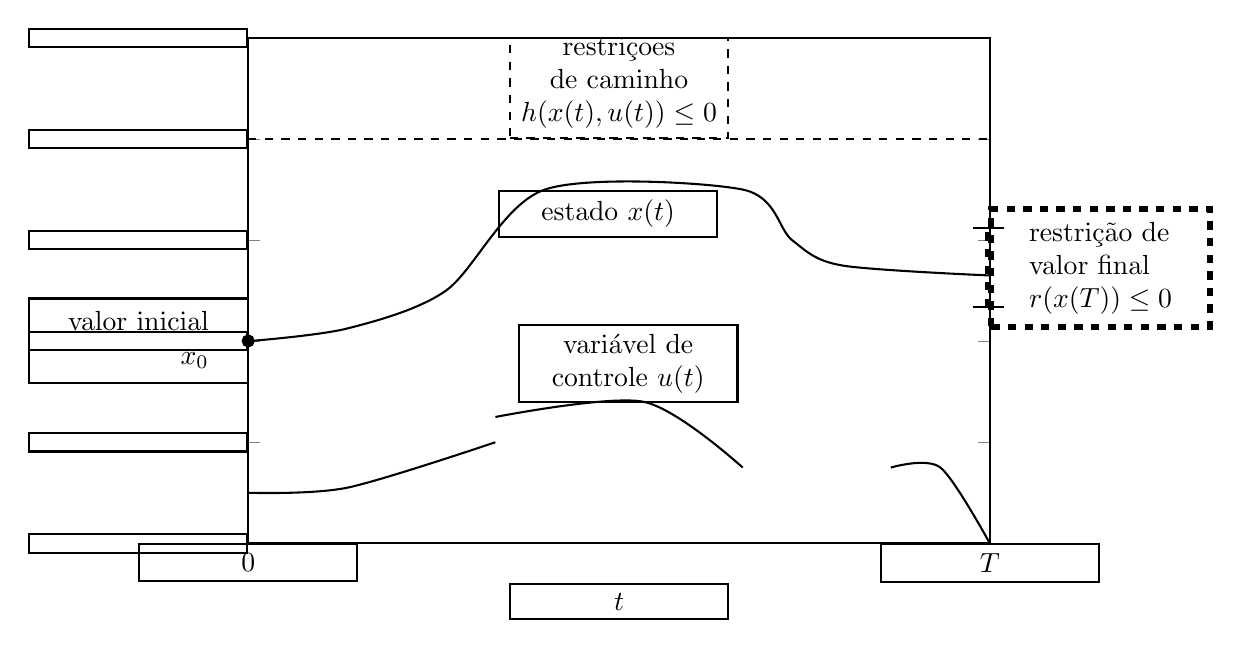
\begin{tikzpicture}
		%\draw [help lines] (-1,-2) grid (12,7);
		\centering
		\begin{axis}[
				width=11cm, height=8cm,
				xmin=0, xmax=15,
				ymin=0, ymax=10,
				xlabel=$t$,
				xtick = {0,15}, xticklabels = {$0$,$T$},
				yticklabels={}]
			\addplot[smooth] plot coordinates {
					(0, 4)
					(2, 4.25)
					(4, 5)
					(6, 7)
					(10, 7)
					(11, 6)
					(12, 5.5)
					(15, 5.3)
				}node[pos=.5, below] {estado $x(t)$};

			\addplot[smooth] plot coordinates {
					(0, 1)
					(2, 1.1)
					(5, 2)
				};
			\addplot[smooth] plot coordinates {
					(5, 2.5)
					(8, 2.8)
					(10, 1.5)
				}node[pos=.5, above] {vari\'{a}vel de controle $u(t)$};
			\addplot[smooth] plot coordinates {
					(10, 0)
					(13, 0)
				};
			\addplot[smooth] plot coordinates {
					(13, 1.5)
					(14, 1.5)
					(15, 0)
				};

			\addplot[dashed, black] coordinates {
					(0,8) (15,8)
				}node[pos=.5, above] {restri\c{c}\~{o}es de caminho $h(x(t),u(t)) \leq 0$};

		\end{axis}
		\filldraw[black] (0,2.57) circle (2pt) node[left] {
				\begin{tabular}{r}
					valor inicial \\$x_0$
				\end{tabular}
			};
		\draw (9.2,3) -- (9.6,3) (9.2,4) -- (9.6,4);
		\draw[dashed,line width=0.75mm] (9.4,3) -- (9.4,4) node[right, pos=.5] {
			\begin{tabular}{l}
				restri\c{c}\~{a}o de \\valor final\\	$r(x(T))\leq 0$
			\end{tabular}
		};
	\end{tikzpicture}
	\caption*{\footnotesize Fonte: Adaptado de }
\end{figure}

\begin{figure}[H]
	\centering
	\caption{Visão geral do métodos numéricos para controle ótimo}
	\label{fig:diagrama_metodos_numericos}
	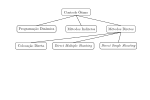
\includegraphics{DescricaoProcesso/Figuras/diagrama_metodos_numericos.png}
	\caption*{\footnotesize Fonte: Adaptado de \citeauthor{article:Diehl}}
\end{figure}

\clearpage